\chapter{Related Work}
\label{chap:relatedwork}
Initially, web IE involved manually written wrappers that catered to specific needs and
information sources \cite{Chawathe1994,Perkowitz1995}. While this provided accuracy in the
information extracted, it required users of such IE systems to have some background in
programming. Later, many wrapper induction tools came about after Kushmerick's paper
\cite{Kushmerick1997}, using several different approaches to the problem (e.g. machine
learning) \cite{Freitag1998,Soderland}. Subsequently, from 2001, systems that required no user
intervention were developed \cite{Chang2001,Crescenzi2002,Arasu2003}. This suggests a trend
toward information extraction systems with less human interaction.
\section{Visual feedback for User annotation}
However, IE systems cannot completely be free of user intervention. ``Supervised approaches,
although require annotation from users, extend well to non-template page extraction if proper
features are selected for extraction rules" \cite{Kayed2006}. Since user annotation is crucial
to web IE, it is important to improve current user interfaces for labelling. Attempts such as
\textit{Lixto}, which has some focus on the user interface aspect of labelling, have tried to
make this process more visual \cite{Baumgartner2001}. Other ways to do this would be to reduce
the amount of sample data required by the system, or to provide a way to give the user
immediate feedback as to what the result of the learnt classifier would be.

There are several commercial systems that also do this, like Mozenda and Needlebase. %cite???
MIT's Solvent is part of a mash-up creation system that also provides users with a similar
visual feedback system. Enabling the users to see what the system will extract helps give a
sense of transparency from the system, and in this way, allows the user to make any required
corrections immediately.

However, the abovementioned systems, with the exception of Needlebase, require users to perform
the changes within a customised browser inside the system. In addition, Mozenda, Needlebase and
Solvent require users to have had experience with programming, as part of their extraction
process requires the user to define the ``flow" of the extraction.

\begin{figure}[htbp]
\begin{center}
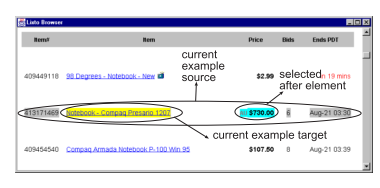
\includegraphics[scale=0.5]{lixto.png} 
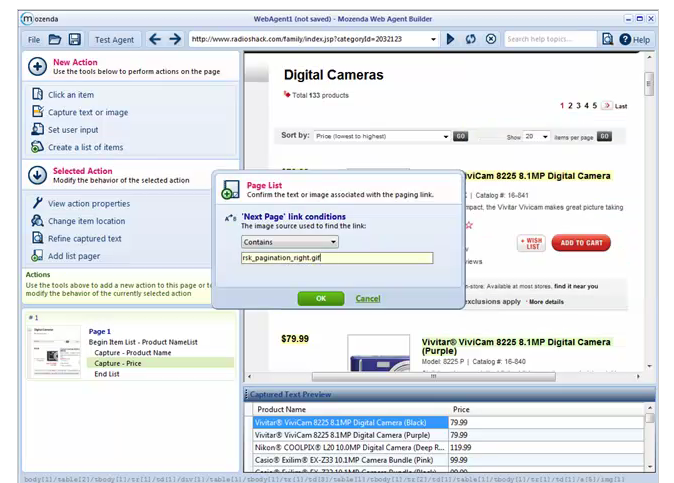
\includegraphics[scale=0.25]{mozenda.png}
\\
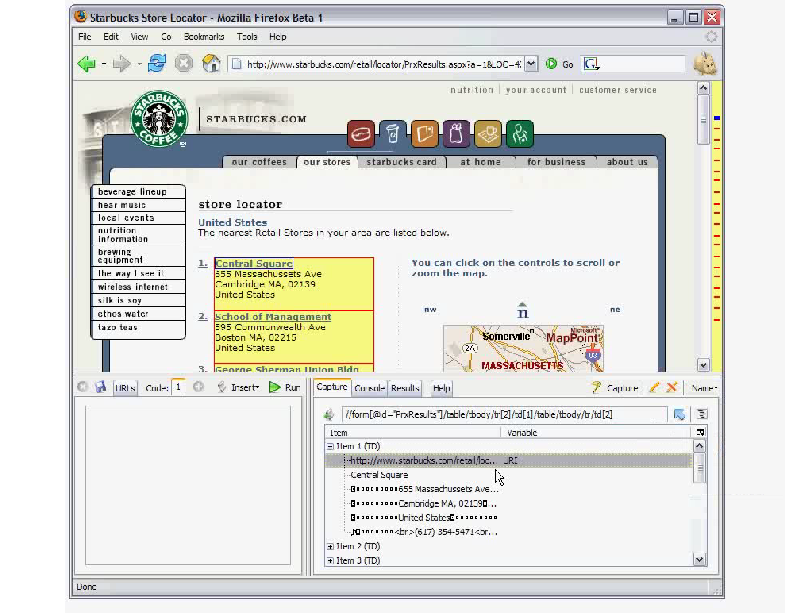
\includegraphics[scale=0.25]{piggybank.png} 
\end{center}

\caption{The \textit{Lixto}, Mozenda and Solvent interfaces.}
\label{fig:lixto}
\end{figure}

\section{Generation of XPath for wrappers}
XPath is a powerful query language commonly used for selecting particular elements in XML
documents. Recently, many scrapers are using XPath as a method of retrieving the relevant
element within an HTML page. This is because its representation of the selected items is
somewhat similar to the way we access directories in our file systems, and also the ubiquity of
XPath as a query language for many HTML parsers makes XPath viable as a tool to retrieve the
relevant elements within a page. However, the process of coming up with the appropriate XPath
lies with the programmer of the scraper. This requires prerequsite knowledge of DOM trees and
XPath, and creating the XPath manually also introduces human error.
	
Methods are available to automate the creation of these XPath queries. A method for extracting
XPaths is described in \cite{Anton2004}. The approach models the DOM Tree as a traversal graph,
and uses this to try to create an XPath that gets the wanted elements for all pages it is given.

Later, \cite{Dalvi2009} explored the approach of developing a tree-edit model of HTML,
modelling changes to a page as a stochastic process, using it to improve wrapper construction
for robustness. The method generates a list of candidate XPaths for a certain selected region
within the page. It used archived data of a given website to calculate its \textit{compute
transformation probability}. Using this, the most robust XPath candidate was selected from the
list. This process, however, required access to archives of older versions of the site. Such
methods of XPath generation do are not immediate, and, for the most part, does not involve a
lot of input from the user, but the drawback of that would be that the user is unaware of what
will be extracted until he/she sees the extracted results.

\section{Robust wrappers}
Another problem faced when trying to automate web IE is having to regenerate or re-implement
the wrapper every time there is a change in the site layout. This is an important problem given
the ease in which templating systems allow pages to be ``themed" and redesigned. Wrappers need
to be robust enough to handle such frequent changes, and be less reliant on the underlying HTML
structure of the page.
	
One method of approaching this was to make use of the visual features of the page. The PARCELS
system is not strictly an information extraction system, but rather, is concerned with dividing
up the page and classifying the resulting blocks correctly. As input, the user is required to
input several example pages with labelled blocks as examples. The system then extracts features
from 2 different aspects of the blocks: Its \textit{lexical} features and its
\textit{stylistic} features. Using both of these the classifier uses a technique called
co-training, machine classified blocks from either view is fed into the training data of the
other view\cite{Lee2004}. The system was then improved to include usage of inter and intra
similarities between pages as features\cite{AikMiang2005}. Gatterbauer also approached the
problem of extracting data from web tables by looking directly at the rendered 2D output,
extracting tables (or grids) within them, and then analysing these in order to extract relevant
information \cite{Gatterbauer2007}.




After studying the drawbacks and advantages of some of the previous work in the area, I hope to
make 2 main contributions with my system:
\begin{enumerate}
	\item Provide an intuitive interface for labelling that is platform agnostic, and takes advantage of the many advancements in Javascript. This will provide the user with an immediate visual feedback as to the items that he/she will be extracting, and at the same time reduce the amount of labelling that needs to be done.
	\item Create a more robust framework for extraction of the selected information using machine learning. The classifier will have less focus on the HTML structural information of the tags in order to be resistant to any layout changes made to the page.
\end{enumerate}

For the rest of the report, I will define users of the system as users who do not have access 
to resources required by current information extraction system. This includes not only the 
hardware and processing power required, but also the time needed for the labelling work done.
Also, I will define robustness as the wrapper's resistance to changes in HTML structure from
the time that the wrapper was derived.






